\documentclass[aspectratio=169]{beamer}

% Je kan het lettertype iets vergroten door hierboven optie ``14pt'' toe te
% voegen.

%==============================================================================
% Aanloop
%==============================================================================

%---------- Vormgeving --------------------------------------------------------

\usetheme{hogent}

% Kies hieronder een achtergrondkleur
%\usecolortheme{hgwhite} % witte achtergrond, zwarte tekst
\usecolortheme{hgblack} % zwarte achtergrond, witte tekst

%---------- Packages ----------------------------------------------------------

\usepackage[english]{babel}      % Nederlandse taal: splitsingen, enz.

\usepackage{booktabs}          % Mooie tabellen
\usepackage{multirow,multicol} % Tabelcellen samenvoegen
\usepackage{eurosym}           % Euro symbool

%\usepackage{animate} % GIFS
\usepackage{media9}
\usepackage{fontspec}
\usepackage{multimedia} % Use multimedia instead of media9
\usepackage{hyperref}


%---------- Commando-definities -----------------------------------------------

%---------- Info over de presentatie ------------------------------------------

\title[AI Judge]{AI judge assistant for recognition of jump rope skills in videos.}
\author{Mike De Decker}
\author[MDD]{Mike {De Decker} (\href{mailto:mikeddecker@hotmail.com}
    {mikeddecker@hotmail.com})}
\date{\today}

%==============================================================================
% Inhoud presentatie
%==============================================================================

\begin{document}

%---------- Titelpagina, inhoudstafel -----------------------------------------

{
\setbeamertemplate{background}[imgletter]
    {dd3-boxes-dark.jpg}{H}

\begin{frame}
    \maketitle
\end{frame}
}

%---------- Corpus ------------------------------------------------------------

\begin{frame}
  \frametitle{Diciplines}

  \hspace{0.1cm}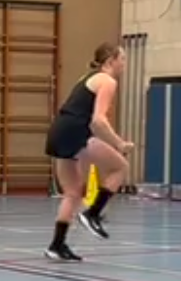
\includegraphics[height=2cm]{speed}
  \hspace{0.1cm}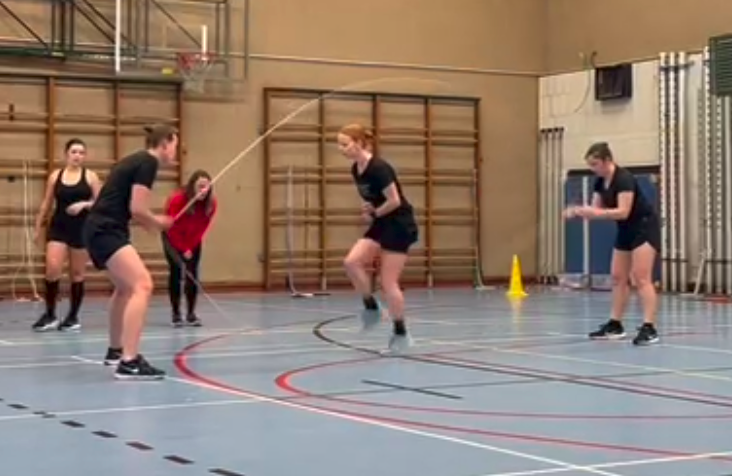
\includegraphics[height=2cm]{ddspeed}
  \hspace{0.1cm}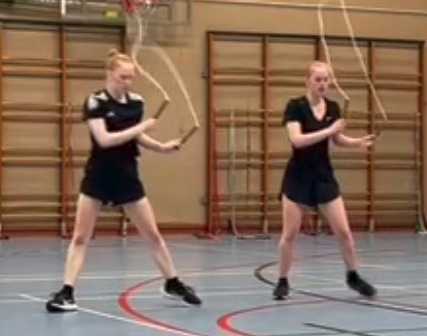
\includegraphics[height=2cm]{sr}
  \hspace{0.1cm}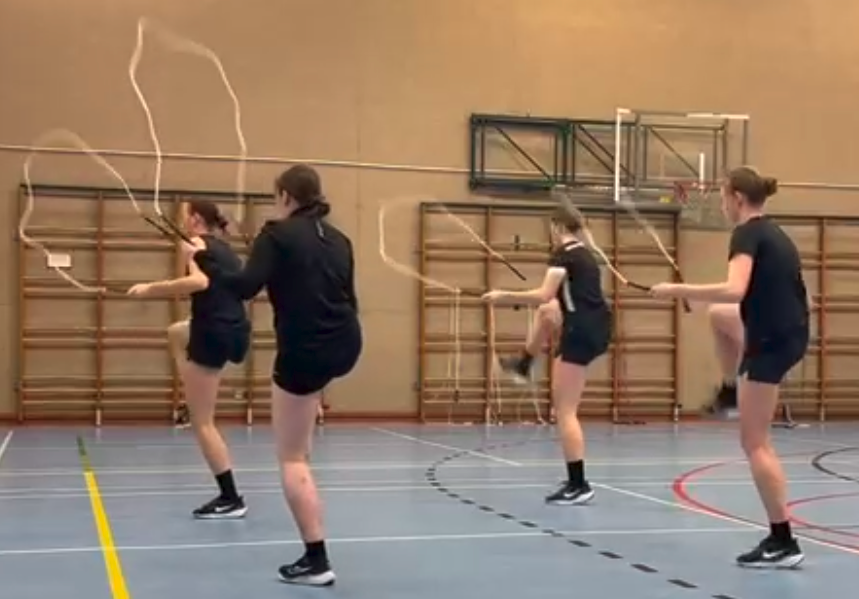
\includegraphics[height=2cm]{sr-team} \\
  \vspace{0.1cm}
  \hspace{0.1cm}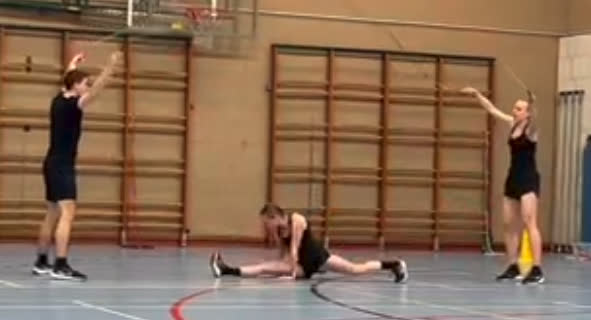
\includegraphics[height=2cm]{dd3}
  \hspace{0.1cm}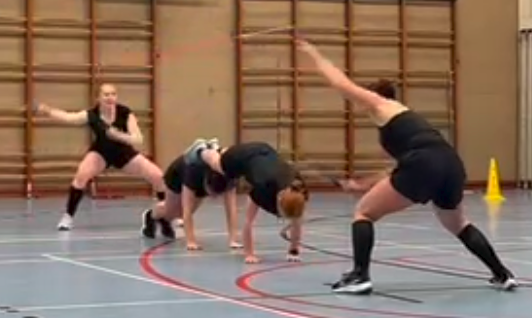
\includegraphics[height=2cm]{dd4}
  \hspace{0.1cm}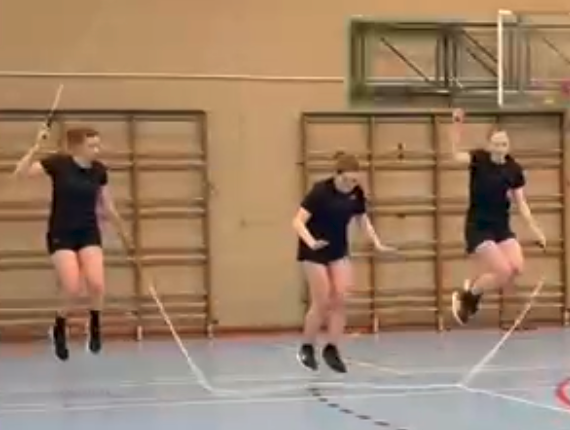
\includegraphics[height=2cm]{cw}

\end{frame}

% \begin{frame}
%   \frametitle{Comparing routines}

%   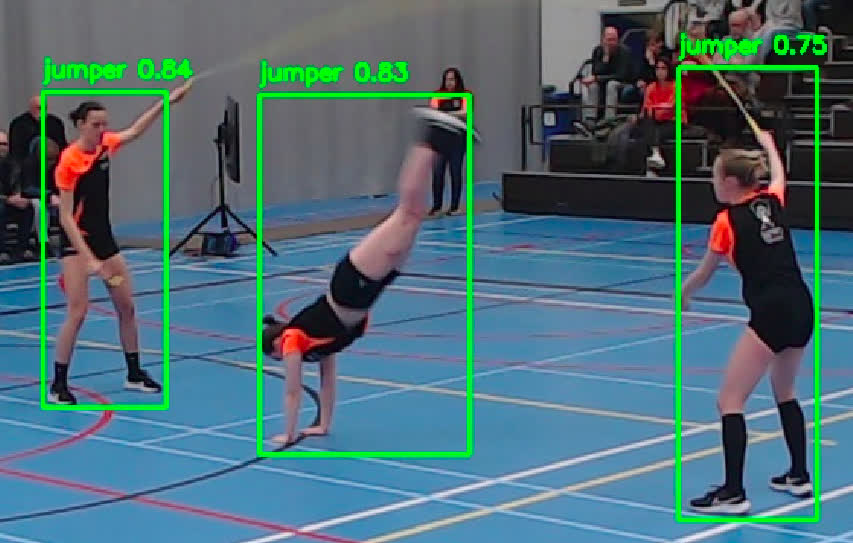
\includegraphics[height=4cm]{dd3-boxes.jpg}
%   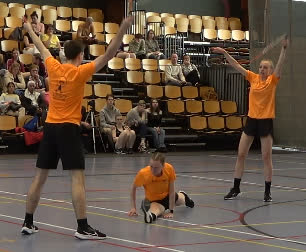
\includegraphics[height=4cm]{dd3-split.jpg}

% \end{frame}

\begin{frame}
  \frametitle{Judges}
  \vspace{-1.5cm}
  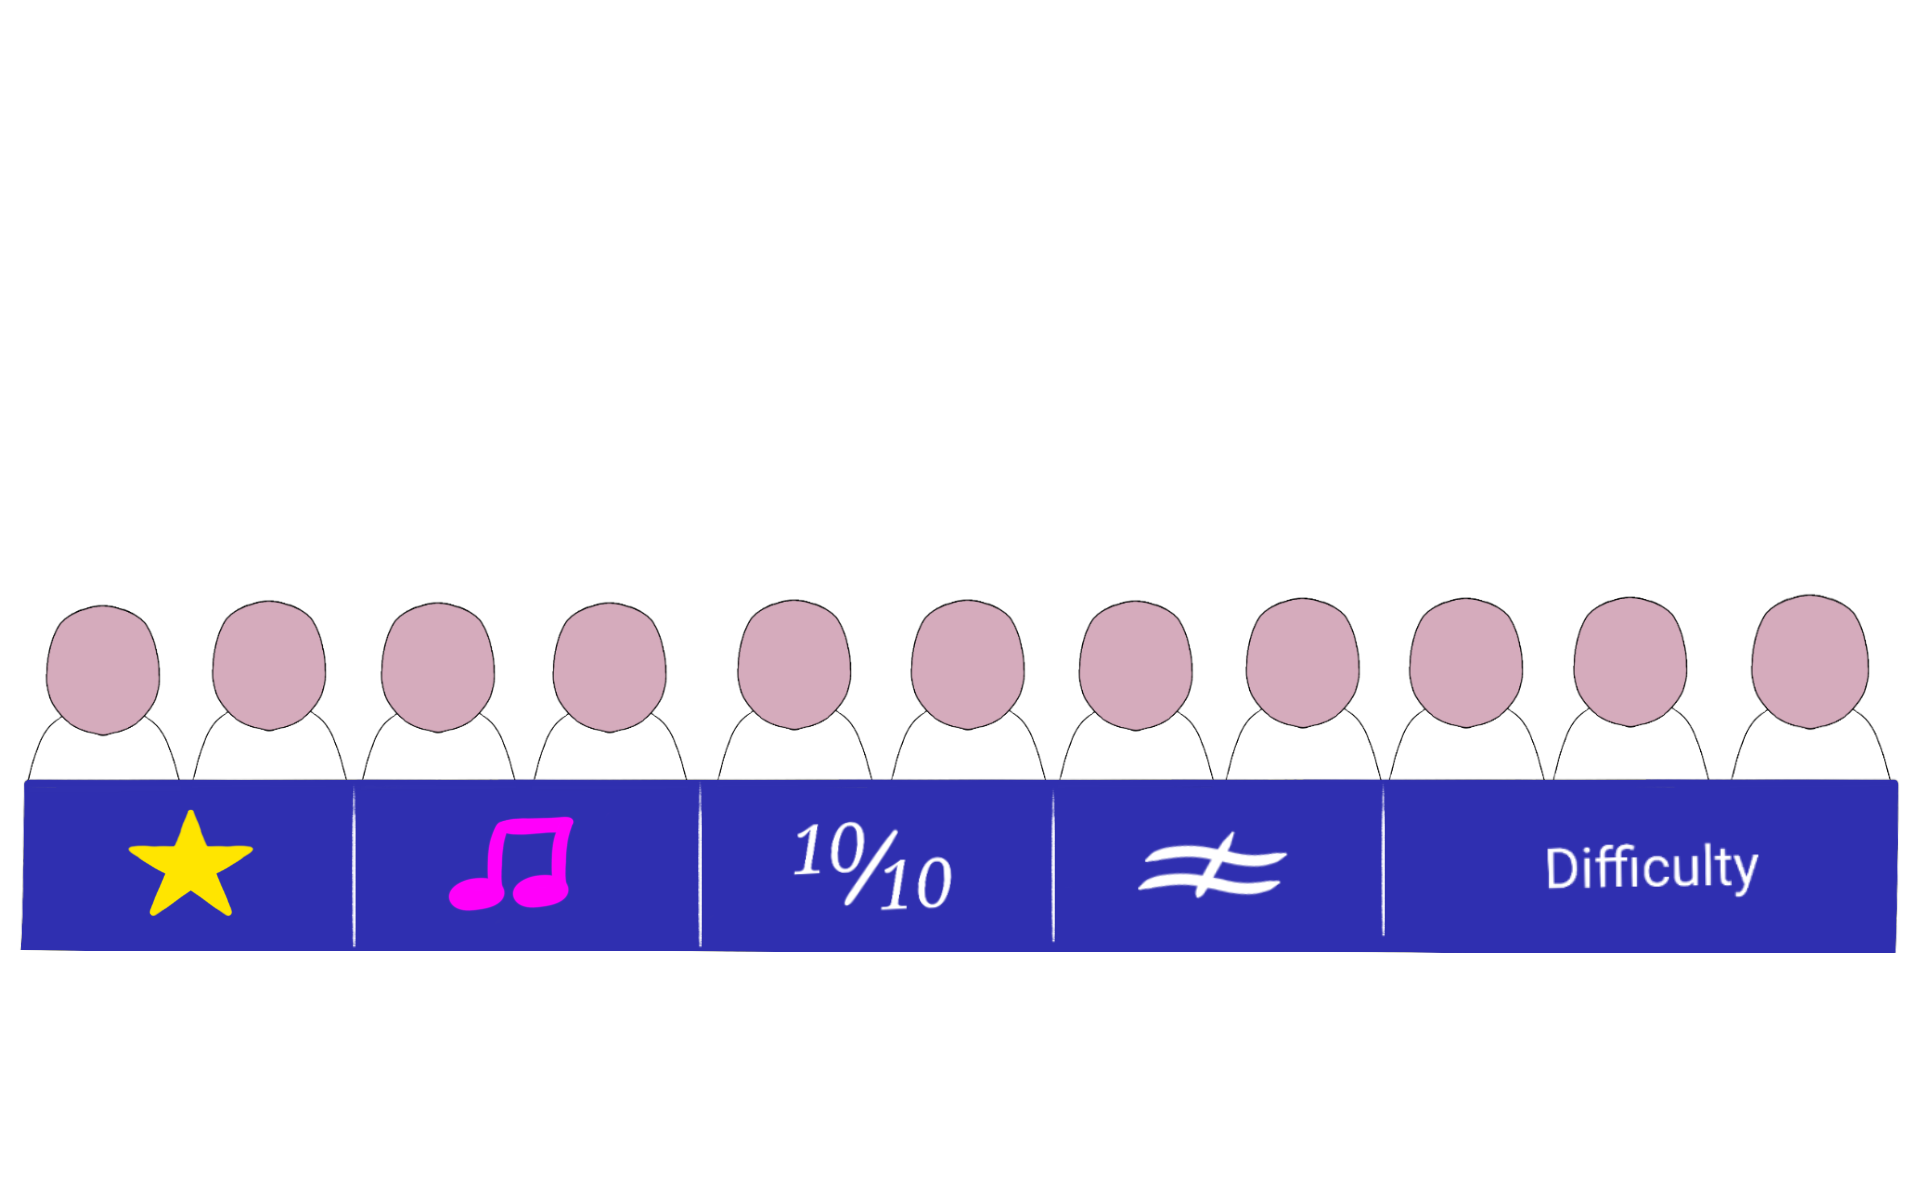
\includegraphics[width=0.9\linewidth]{judges}
  
  % TODO : add cine diffusion link if kept
\end{frame}

\begin{frame}
  \frametitle{Scoring difficulty.}
  \vspace{-0.3cm}
  Using levels [1 -> 8]
  \vspace{0.2cm}

  \begin{columns}[c]
  
    \column{.55\textwidth}
    \hspace{0.2cm} 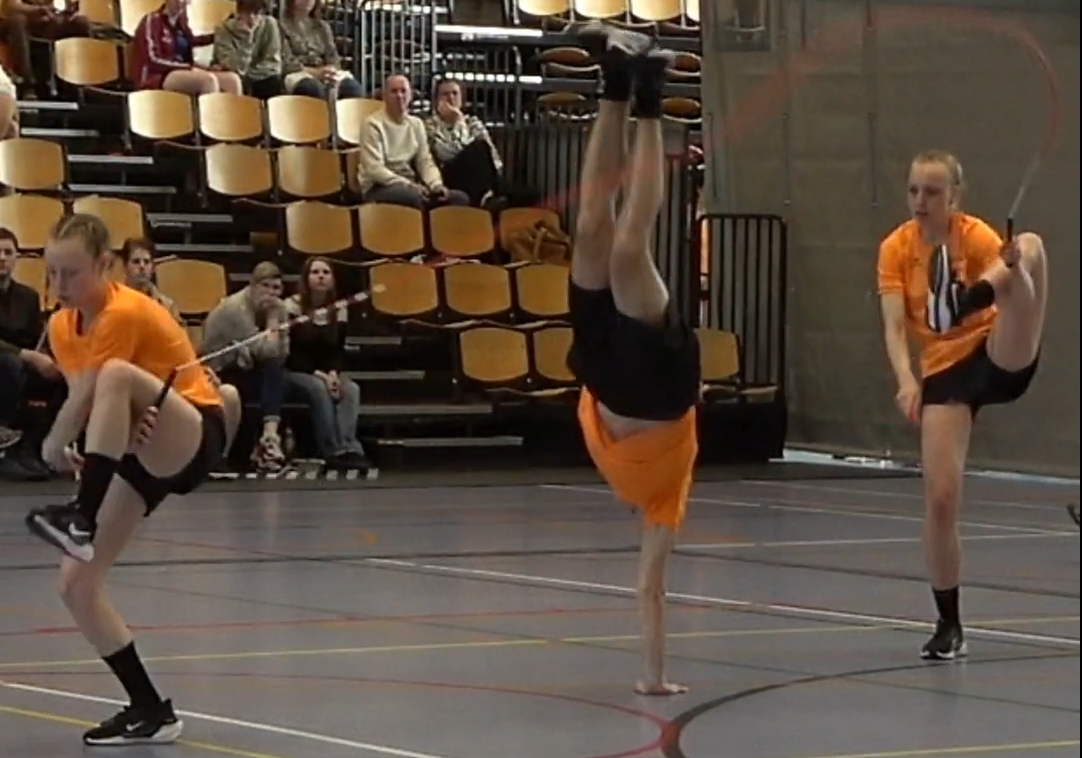
\includegraphics[width=0.85\linewidth]{dd3-1h-hfrog-toad-bw-crouger}

    \column{.45\textwidth}
    Base skill level \\
    + \\
    Turner restrictions \\
    + \\
    Nr of rotations \\
    + \\
    Modifiers (one hand, body rotations...)

  \end{columns}
\end{frame}

\begin{frame}
  \frametitle{AI Judge assistant}

  \begin{columns}[c]
  
    \column{.75\textwidth}
    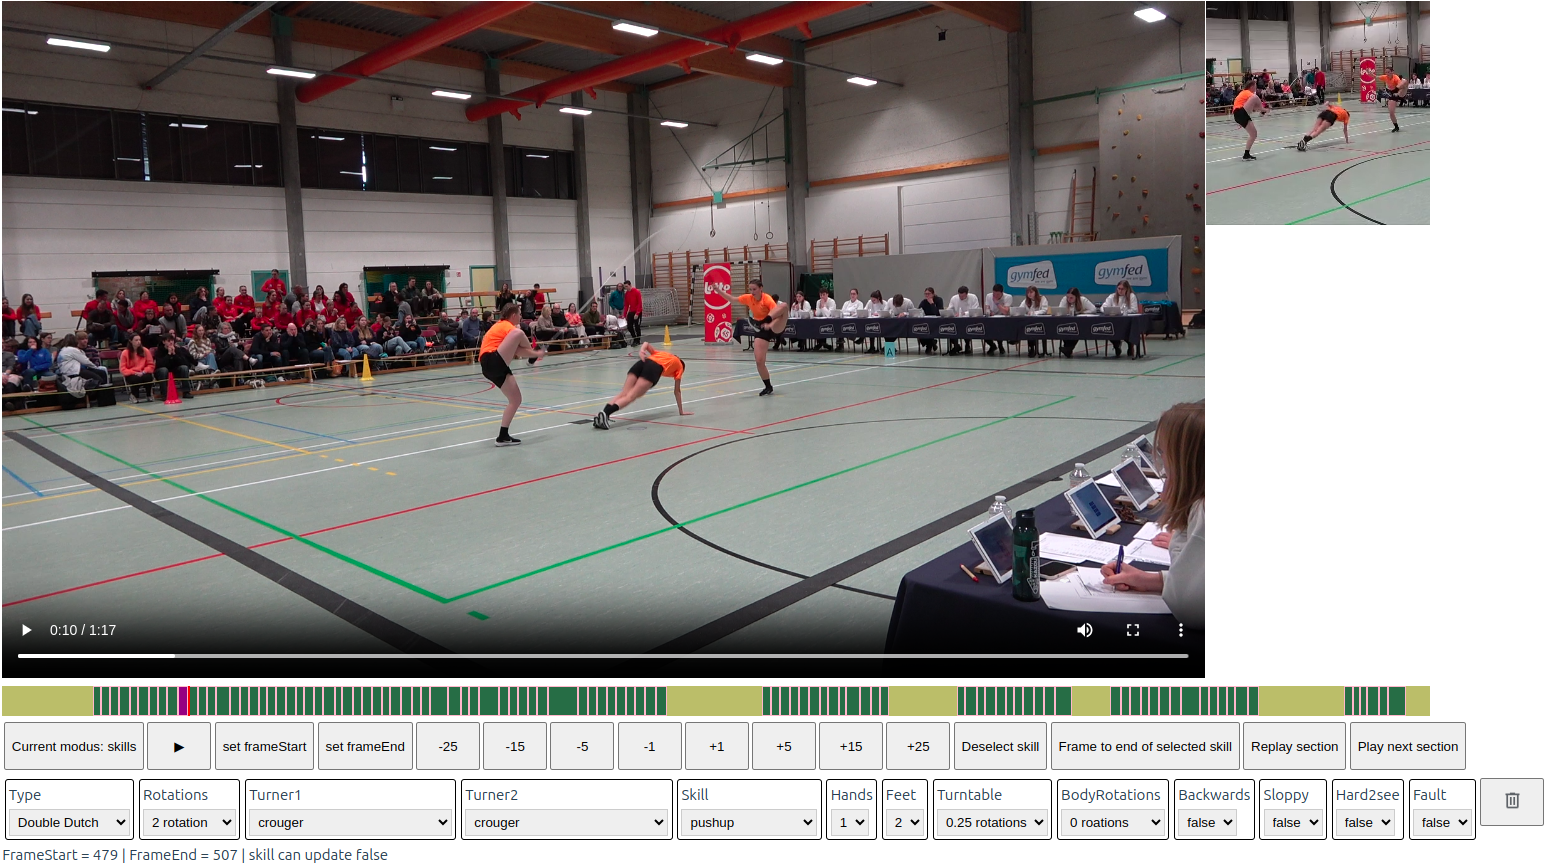
\includegraphics[width=1.0\linewidth]{label-video}

    \column{.25\textwidth}
    \vspace{-1.0cm}
    \begin{enumerate}
      \item localize
      \item segment
      \item recognition
    \end{enumerate}

  \end{columns}
\end{frame}

\begin{frame}
  \frametitle{AI Judge assistant}

  \begin{columns}[c]
    \column{.33\textwidth}
    \centering{Localize}
    \column{.33\textwidth}
    \centering{Segment}
    \column{.33\textwidth}
    \centering{Recognize}
  \end{columns}

  \begin{columns}[c]
  
    \column{.33\textwidth}
    \begin{center}
      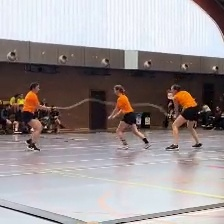
\includegraphics[width=0.8\linewidth]{ai-judge-localize-crop}
    \end{center}
    
    \column{.33\textwidth}
    \begin{center}
      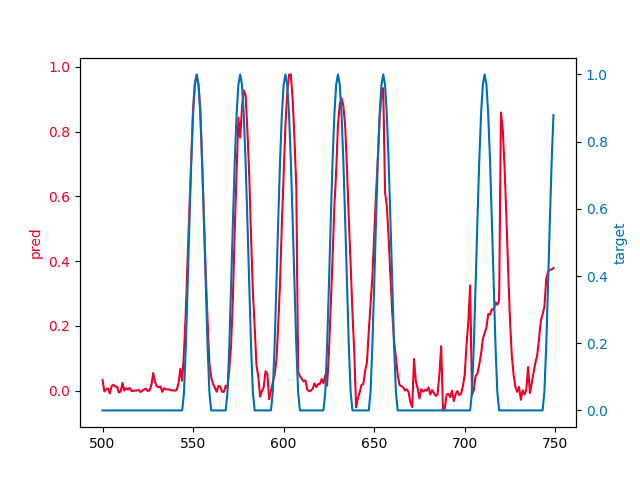
\includegraphics[width=1.0\linewidth]{ai-judge-segment-plot}
    \end{center}
    % \vspace{0.kcm}
    \begin{center}
      
\includegraphics[width=0.8\linewidth]{ai-judge-segments}
    \end{center}

    \column{.33\textwidth}
    
    \begin{center}
        cartwheel \\
        handstand \\
        2 rotations \\
        1 hand \\
        2 feet \\
        ... 
    \end{center}
      
  \end{columns}


\end{frame}

\begin{frame}{Video example}
  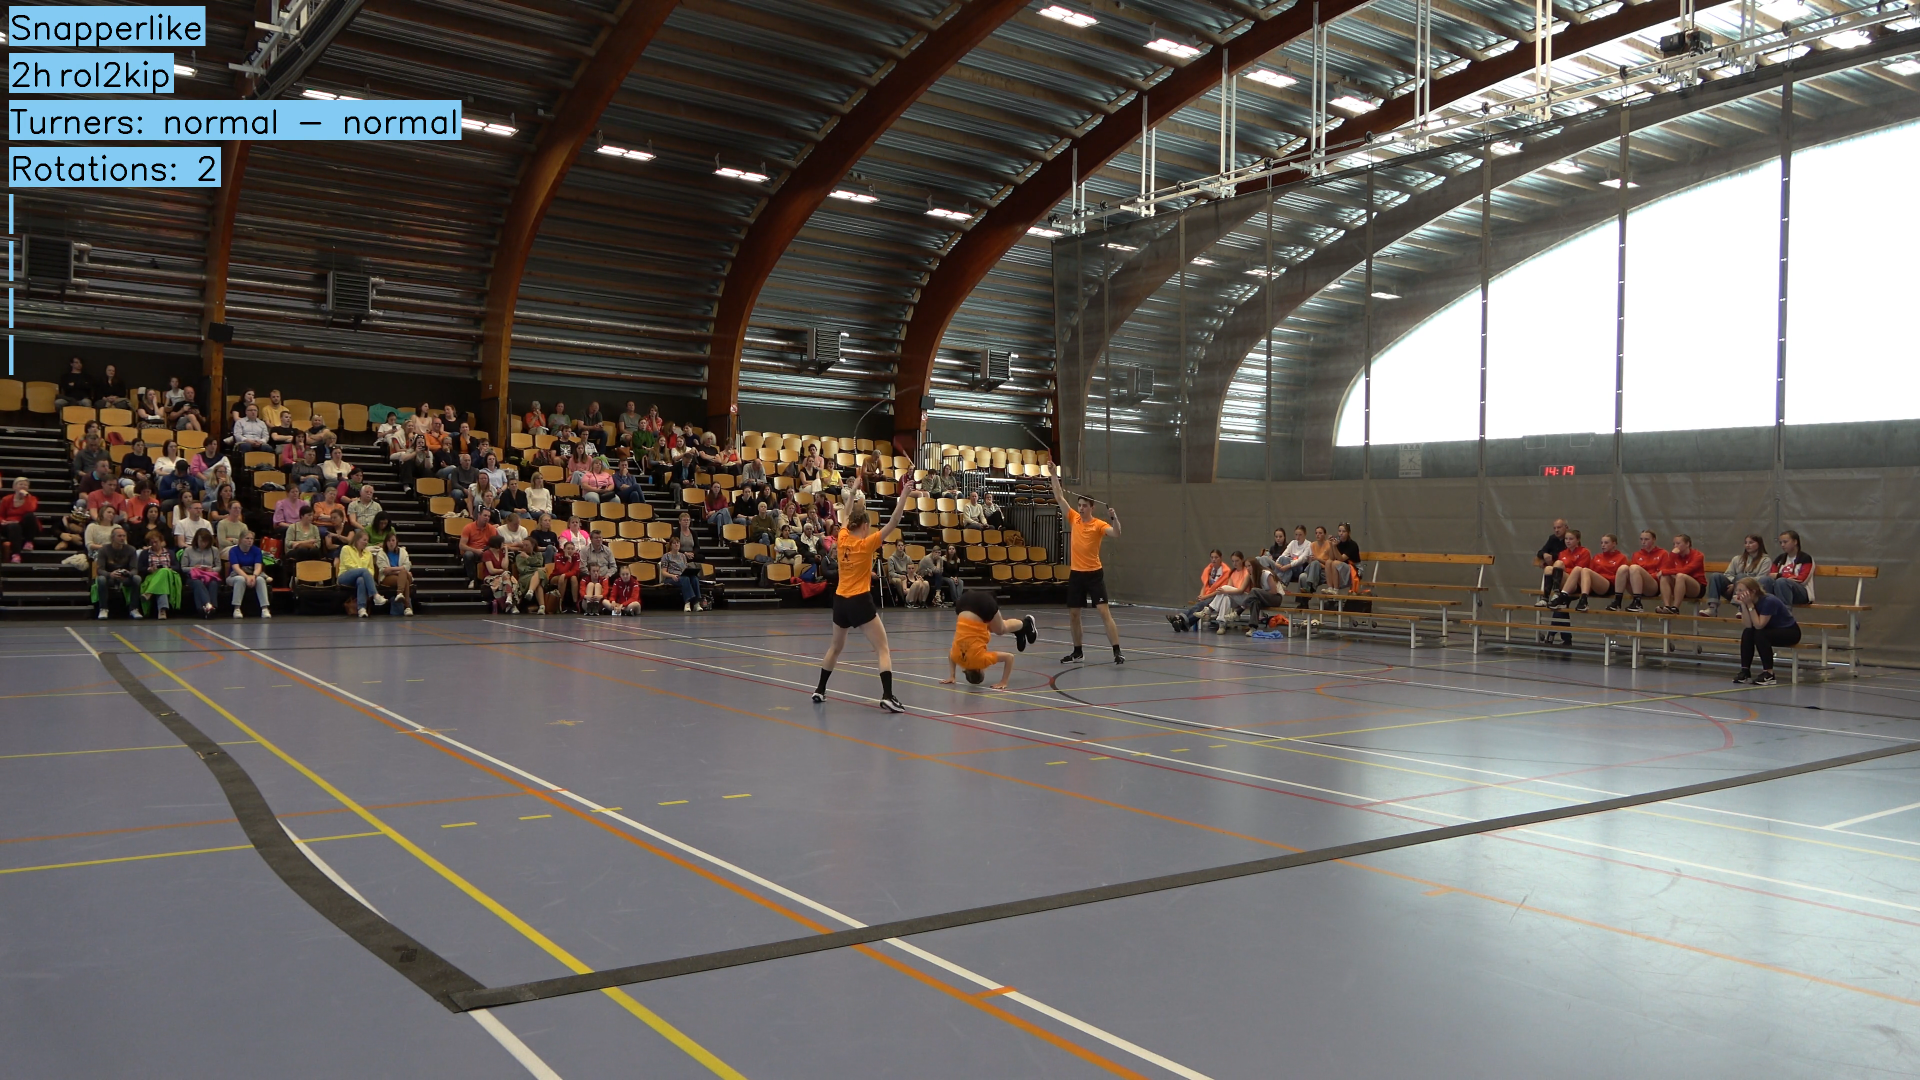
\includegraphics[width=0.6\linewidth]{dd3-predicted-skill} 
  
  % \href{run:dd3-annotated.mp4}{\beamergotobutton{Click to play the video}}
  % \pdfcatalog{/OpenAction << /S /JavaScript /JS (app.openURI('file:./dd3-annotated.mp4', 'newWindow');) >>}
  
  \hypertarget{autoplay}{} % A dummy target
  \href{run:dd3-annotated.mp4}{\beamergotobutton{Click to play the video}}

  % JavaScript to auto-trigger the click
  \pdfstringdefDisableCommands{%
    \def\insertbuttonlink{\JavaScript{app.launchURL("dd3-annotated.mp4", true);}}%
  }

\end{frame}


\end{document}
